%%%%%%%%%%%%%%%%%%%%%%%%%%%%%%%%%%%%%%%%%%%%%%%%%%%%%%%%%%%%%%%%%%%%%%%%%%%%%%%%%%%%%%%%%%%%%%%%
%
% CSCI 1430 Written Question Template
%
% This is a LaTeX document. LaTeX is a markup language for producing documents.
% Your task is to answer the questions by filling out this document, then to
% compile this into a PDF document.
%
% TO COMPILE:
% > pdflatex thisfile.tex
%
% If you do not have LaTeX and need a LaTeX distribution:
% - Departmental machines have one installed.
% - Personal laptops (all common OS): http://www.latex-project.org/get/
%
% If you need help with LaTeX, come to office hours. Or, there is plenty of help online:
% https://en.wikibooks.org/wiki/LaTeX
%
% Good luck!
% Srinath and the 1430 staff
%
%%%%%%%%%%%%%%%%%%%%%%%%%%%%%%%%%%%%%%%%%%%%%%%%%%%%%%%%%%%%%%%%%%%%%%%%%%%%%%%%%%%%%%%%%%%%%%%%
%
% How to include two graphics on the same line:
%
% \includegraphics[width=0.49\linewidth]{yourgraphic1.png}
% \includegraphics[width=0.49\linewidth]{yourgraphic2.png}
%
% How to include equations:
%
% \begin{equation}
% y = mx+c
% \end{equation}
%
%%%%%%%%%%%%%%%%%%%%%%%%%%%%%%%%%%%%%%%%%%%%%%%%%%%%%%%%%%%%%%%%%%%%%%%%%%%%%%%%%%%%%%%%%%%%%%%%

\documentclass[11pt]{article}

\usepackage[english]{babel}
\usepackage[utf8]{inputenc}
\usepackage[colorlinks = true,
            linkcolor = blue,
            urlcolor  = blue]{hyperref}
\usepackage[a4paper,margin=1.5in]{geometry}
\usepackage{stackengine,graphicx}
\usepackage{fancyhdr}
\usepackage{amsmath}
\usepackage{amssymb}
\usepackage{enumerate}
\setlength{\headheight}{15pt}
\usepackage{microtype}
\usepackage{times}
\usepackage{booktabs}
\usepackage[shortlabels]{enumitem}
\setlist[enumerate]{topsep=0pt}

% python code format: https://github.com/olivierverdier/python-latex-highlighting
\usepackage{pythonhighlight}

\frenchspacing
\setlength{\parindent}{0cm} % Default is 15pt.
\setlength{\parskip}{0.3cm plus1mm minus1mm}

\pagestyle{fancy}
\fancyhf{}
\lhead{Homework 3 Questions}
\rhead{CSCI 1430}
\lfoot{\textcolor{red}{Only
\ifcase\thepage
\or A1
\or A1
\or A2
\or A2
\or A3
\or A4
\or A4
\or Q5
\or A5
\or A6
\or A6
\or feedback
\else
EXTRA PAGE ADDED
\fi
should be on this page
}}
\rfoot{\thepage/11}

\date{}

\title{\vspace{-1cm}Homework 3 Questions}


\begin{document}
\maketitle
\vspace{-2cm}
\thispagestyle{fancy}

\section*{Instructions}
\begin{itemize}
  \item 6 questions.
  \item Write code where appropriate; feel free to include images or equations.
  \item Please make this document anonymous.
  \item This assignment is \textbf{fixed length}, and the pages have been assigned for you in Gradescope. As a result, \textbf{please do NOT add any new pages}. We will provide ample room for you to answer the questions. If you \emph{really} wish for more space, please add a page \emph{at the end of the document}.
  \item \textbf{We do NOT expect you to fill up each page with your answer.} Some answers will only be a few sentences long, and that is okay.
\end{itemize}

\section*{Questions}

%%%%%%%%%%%%%%%%%%%%%%%%%%%%%%%%%%%

\paragraph{Q1:} Given a stereo pair of cameras:
\begin{enumerate} [(a)]
\item Briefly describe triangulation (using images might be helpful).
\item Why is it not possible to find an absolute depth for each point when we don't have calibration information for our cameras?
\end{enumerate}

%%%%%%%%%%%%%%%%%%%%%%%%%%%%%%%%%%%
\paragraph{A1:} Your answer here.
% Uncomment the stencil below and fill in your solution.

% \begin{enumerate}[(a)]

% \item

% \item

% \end{enumerate}

%%%%%%%%%%%%%%%%%%%%%%%%%%%%%%%%%%%
% Please leave the pagebreak
\pagebreak
\paragraph{A1 (continued):} Your answer here.


%%%%%%%%%%%%%%%%%%%%%%%%%%%%%%%%%%%
% Please leave the pagebreak
\pagebreak
\paragraph{Q2:} In lecture, you've learned that cameras can be represented by intrinsic and extrinsic matrices. These matrices can then be used to calculate the projections of points with 3D world coordinates onto 2D images. 
\begin{enumerate} [(a)]
\item For each of the following camera specifications, fill in its intrinsic and extrinsic matrices. Then perform the multiplications and homogenize to find the 2D coordinates of the projected point on the image.
\begin{enumerate} [(i)]

\item A camera with focal length in both $x$ and $y$ directions of $1$, and\\
no skew, translation, or rotation.
\vspace{-0.3cm}
\begin{align}
    \begin{pmatrix} 
    \_\_ & \_\_ & $0$ \\ 
    $0$ & \_\_ & $0$ \\ 
    $0$ & $0$ & $1$ \end{pmatrix} *
    \begin{pmatrix} 
    \_\_ & \_\_ & \_\_ & \_\_ \\ 
    \_\_ & \_\_ & \_\_ & \_\_ \\ 
    \_\_ & \_\_ & \_\_ & \_\_ \end{pmatrix} * 
    \begin{pmatrix} 
    $30$ \\ 
    $-20$ \\ 
    $10$ \\ 
    $1$ \end{pmatrix}
    = \begin{pmatrix}  \_\_ \\ \_\_ \\ \_\_ \end{pmatrix}
    = \_\_ * \begin{pmatrix}  \_\_ \\ \_\_ \\ $1$ \end{pmatrix}
\end{align}

\item A camera with focal length in both $x$ and $y$ directions of $2$,\\a translation of $5$ along the x-axis, and\\ no skew or rotation.
\vspace{-0.3cm}
\begin{align}
    \begin{pmatrix} 
    \_\_ & \_\_ & $0$ \\ 
    $0$ & \_\_ & $0$ \\ 
    $0$ & $0$ & $1$ \end{pmatrix} *
    \begin{pmatrix} 
    \_\_ & \_\_ & \_\_ & \_\_ \\ 
    \_\_ & \_\_ & \_\_ & \_\_ \\ 
    \_\_ & \_\_ & \_\_ & \_\_ \end{pmatrix} * 
    \begin{pmatrix} 
    $30$ \\ 
    $-20$ \\ 
    $10$ \\ 
    $1$ \end{pmatrix}
    = \begin{pmatrix}  \_\_ \\ \_\_ \\ \_\_ \end{pmatrix}
    = \_\_ * \begin{pmatrix}  \_\_ \\ \_\_ \\ $1$ \end{pmatrix}
\end{align}

\end{enumerate}
\item Compare the two image coordinates you've calculated in parts a and b. Explain how each parameter affects the final image coordinate. (2-3 sentences)

\item In the questions folder, we've provided stencil code for a camera simulation in camera\_simulation.py. Given a projection matrix, the simulator visualizes an image that a camera would produce. Please implement calculate\_projection\_matrix() by calculating the projection matrix using the parameters given in the code (see stencil for more detail). Paste your code for this function and attach a screenshot of the working demo once you finish!

\end{enumerate}

%%%%%%%%%%%%%%%%%%%%%%%%%%%%%%%%%%%
\paragraph{A2:} Your answer here.
% Uncomment the stencil below and fill in your solution.

% \begin{enumerate}[(b)]

% \item

% \end{enumerate}

% \begin{enumerate}[(c)]

% \item

% \begin{python}
% # Your code here
% \end{python}

% \includegraphics[width=0.5\linewidth]{yourscreenshot.png}

% \end{enumerate}

%%%%%%%%%%%%%%%%%%%%%%%%%%%%%%%%%%%
% Please leave the pagebreak
\pagebreak
\paragraph{A2 (continued):} Your answer here.


%%%%%%%%%%%%%%%%%%%%%%%%%%%%%%%%%%%

% Please leave the pagebreak
\pagebreak
\paragraph{Q3:} In two-view camera geometry, what do the following epipolar lines say about the cameras' relative positions?:
\begin{enumerate}[(a)]
\item radiate out of a point on the image plane,

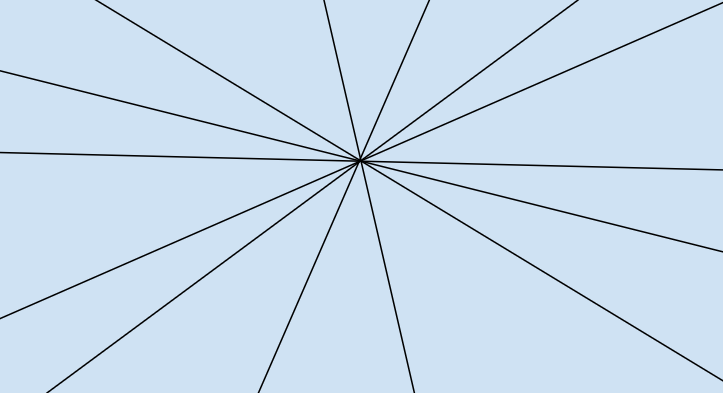
\includegraphics[width = 0.25\linewidth]{q3-a.PNG}
\item converge to a point outside of the image plane, and


\includegraphics[width = 0.25\linewidth]{q3-b.PNG}
\end{enumerate}

We highly recommend using this \href{https://browncsci1430.github.io/webpage/demos/stereo_camera_visualization/index.html}{interactive demo} to explore the different scenarios and get a better feel for epipolar geometry.
\begin{enumerate}[(c)]
\item What might you need to change about your calculations if you obtained the following epipolar lines? (Hint: check slides from lecture 9)

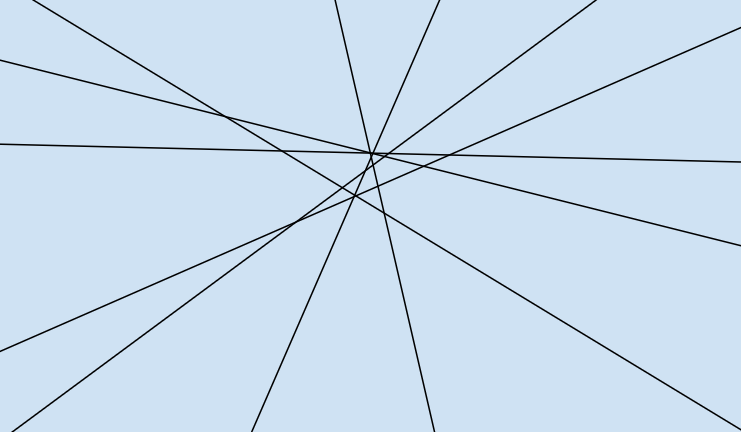
\includegraphics[width = 0.25\linewidth]{q3-c.PNG}
\end{enumerate}


%%%%%%%%%%%%%%%%%%%%%%%%%%%%%%%%%%%
\paragraph{A3:} Your answer here.
% Uncomment the stencil below and fill in your solution.

% \begin{enumerate}[(a)]

% \item

% \item

% \item

% \end{enumerate}

%%%%%%%%%%%%%%%%%%%%%%%%%%%%%%%%%%%
\pagebreak
\paragraph{Q4:}
Suppose that we have the following three datasets of an object of unknown geometry:
\begin{enumerate}[(a)]
\item A video circling the object;
\item An stereo pair of calibrated cameras capturing two images of the object; and
\item Two images we take of the object at two different camera poses (position and orientation) using the same camera but with different lens zoom settings.
\end{enumerate}

\begin{enumerate}
\item For each of the above setups, decide if we are able to find/calculate the essential matrix, the fundamental matrix, or both. \\
\emph{LaTeX:} To fill in boxes, replace `\textbackslash square' with `\textbackslash blacksquare' for your answer. \\ \\
(a)
\begin{tabular}[h]{lc}
\toprule
Essential Matrix & $\square$ \\
Fundamental Matrix & $\square$ \\
Both & $\square$ \\
\end{tabular} \\
(b)
\begin{tabular}[h]{lc}
\toprule
Essential Matrix & $\square$ \\
Fundamental Matrix & $\square$ \\
Both & $\square$ \\
\end{tabular} \\
(c)
\begin{tabular}[h]{lc}
\toprule
Essential Matrix & $\square$ \\
Fundamental Matrix & $\square$ \\
Both & $\square$ \\
\bottomrule
\end{tabular}
\item State an advantage and disadvantage of using each setup for depth reconstruction; and
\item Name an application scenario for each of the different setups.
\end{enumerate}

%%%%%%%%%%%%%%%%%%%%%%%%%%%%%%%%%%%
\paragraph{A4:} Your answer here.
% Uncomment the stencil below and fill in your solution.

% \begin{enumerate}[(a)]

% \item

% \item

% \item

% \end{enumerate}

%%%%%%%%%%%%%%%%%%%%%%%%%%%%%%%%%%%
% Please leave the pagebreak
\pagebreak
\paragraph{A4 (continued):} Your answer here.


%%%%%%%%%%%%%%%%%%%%%%%%%%%%%%%%%%%
\pagebreak
\paragraph{Q5 (Linear algebra/numpy question):}
Suppose we have a quadrilateral $ABCD$ and a transformed version $A'B'C'D'$ as seen in the image below.

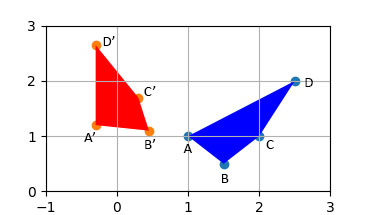
\includegraphics[width=8cm]{quadrilaterals.jpg}

\begin{equation}
\begin{split}
A&=(1, 1)\\
B&=(1.5, 0.5)\\
C&=(2, 1)\\
D&=(2.5, 2)
\end{split}
\quad\quad\quad
\begin{split}
A'&=(-0.3, 1.3)\\
B'&=(0.5, 1.1)\\
C'&=(0.3, 1.8)\\
D'&=(-0.3, 2.6)
\end{split}
\end{equation}

Let's assume that each point in $ABCD$ was approximately mapped to its corresponding point in $A'B'C'D'$ by a $2\times2$ transformation matrix $M$.

e.g. if $A = \begin{pmatrix} x \\ y \end{pmatrix}$ and $A' = \begin{pmatrix} x' \\ y' \end{pmatrix}$, and $\boldsymbol{M} = \begin{pmatrix} m_{1,1} & m_{1,2} \\ m_{2,1} & m_{2,2} \end{pmatrix}$

then $\begin{pmatrix} m_{1,1} & m_{1,2} \\ m_{2,1} & m_{2,2} \end{pmatrix} * \begin{pmatrix} x \\ y \end{pmatrix} \approx \begin{pmatrix} x' \\ y' \end{pmatrix}$

We would like to approximate $\boldsymbol{M}$ using least squares for linear regression.

\begin{enumerate}[(a)]
\item Rewrite the equation $\boldsymbol{M}x \approx x'$ into a pair of linear equations. We have provided you with a template of what they should look like below.

\item Use the equations you wrote for part (a) and coordinate values for $ABCD$ and $A'B'C'D'$ to construct a matrix $\boldsymbol{Q}$ and column vector $b$ that satisfy
\begin{align}
    \boldsymbol{Q}*\begin{pmatrix} m_{1,1} \\ m_{1,2} \\ m_{2,1} \\ m_{2,2} \\ \end{pmatrix} = b
\end{align}

We have provided you with a template of what they should look like below.

\emph{Hint:} You have a pair of equations for each $x$-$x'$ correspondence, giving you $8$ rows in $\boldsymbol{Q}$ and $b$. If you're having trouble, try writing out the equations for each pair of points like in part (a).

\emph{Note:} Systems of linear equations are typically written in the form $\boldsymbol{A}x=b$, but since we have already defined $A$ and $x$, we're writing it as $\boldsymbol{Q}m=b$

\item Our problem is now over-constrained, so we want to find values for $m_{i,j}$ that minimize the squared error between approximated values and real values, or $||\boldsymbol{Q}m-b||_2$. To do this we use singular value decomposition to find the pseudoinverse of $\boldsymbol{Q}$, written as $\boldsymbol{Q}^\dagger$. We then multiply it by both sides, giving us $\boldsymbol{Q}^\dagger \boldsymbol{Q}m = \boldsymbol{Q}^\dagger b \quad\Rightarrow\quad m \approx \boldsymbol{Q}^\dagger b$.

Thankfully, the computer can do all of this for us! \texttt{numpy.linalg.lstsq()} takes in our $\boldsymbol{Q}$ matrix and $b$ vector, and returns approximations for $m$. Plug the values you wrote in part (b) into that function and write the returned $\boldsymbol{M}$ matrix here.
\end{enumerate}

%%%%%%%%%%%%%%%%%%%%%%%%%%%%%%%%%%%
\paragraph{A5:} Your answer here.
% Uncomment the stencil below and fill in your solution.

\begin{enumerate}[(a)]

\item Replace each of the `$\_\_$' below with $x, y, x', y',$ or $0$.
\begin{align}
\begin{cases}
    \_\_m_{1,1} + \_\_m_{1,2} + \_\_m_{2,1} + \_\_m_{2,2} = \_\_ \\
    \_\_m_{1,1} + \_\_m_{1,2} + \_\_m_{2,1} + \_\_m_{2,2} = \_\_
\end{cases}
\end{align}

\item Replace each of the `$\_\_$' below with a $0$ or a coordinate value from $ABCD$ and $A'B'C'D'$.
\begin{align}
    \begin{pmatrix} \_\_ & \_\_ & \_\_ & \_\_ \\ \_\_ & \_\_ & \_\_ & \_\_ \\ \_\_ & \_\_ & \_\_ & \_\_ \\ \_\_ & \_\_ & \_\_ & \_\_ \\ \_\_ & \_\_ & \_\_ & \_\_ \\ \_\_ & \_\_ & \_\_ & \_\_ \\ \_\_ & \_\_ & \_\_ & \_\_ \\ \_\_ & \_\_ & \_\_ & \_\_\end{pmatrix} *\begin{pmatrix} m_{1,1} \\ m_{1,2} \\ m_{2,1} \\ m_{2,2} \\ \end{pmatrix} = \begin{pmatrix} \_\_ \\ \_\_ \\ \_\_ \\ \_\_ \\ \_\_ \\ \_\_ \\ \_\_ \\ \_\_ \end{pmatrix}
\end{align}

\item Replace each of the `$\_\_$' below with the value of $m_{i, j}$.
\begin{align}
    M = \begin{pmatrix} m_{1,1} & m_{1,2} \\ m_{2,1} & m_{2,2} \end{pmatrix} = \begin{pmatrix} \_\_ & \_\_ \\ \_\_ & \_\_ \end{pmatrix}
\end{align}

\end{enumerate}

%%%%%%%%%%%%%%%%%%%%%%%%%%%%%%%%%%%

\pagebreak
\paragraph{Q6:} Goal: Be aware of some of the implicit assumptions that shape our views and decisions regarding photography technology and discuss how some of the challenges in photography are part of a longer history of technological development and social change. 

A common problem in photography and videography is properly calibrating lighting for a camera to capture a wide variety of skin tones. This issue stems from an inherited bias built into photography that light skin as the norm. Watch \href{https://www.youtube.com/watch?v=d16LNHIEJzs}{this video} on Kodak’s Shirley Card and answer the following questions.  
\begin{enumerate}[(a)]

    \item
    What kind of harm can come to marginalized or minority populations that aren't considered when building imaging technology? Are we seeing any of these effects today? (3--4 sentences)

    \item
    Read about how some researchers are trying to take the racial bias out of computer vision applications \href{https://news.northeastern.edu/2021/02/22/humans-are-trying-to-take-bias-out-of-facial-recognition-programs-its-not-working-yet/}{here}. If you were developing and launching a new camera, what steps would you take to eliminate possible racial bias? (3--4 sentences)
    
    \item
    It took chocolate and wood corporations complaining that their products couldn’t be photographed correctly for Kodak to adjust its film to be more inclusive of other skin tones. Who should be involved in shaping the direction of new photography developments in the future (companies, developers, interest groups etc)? (3--4 sentences)


\end{enumerate}


%%%%%%%%%%%%%%%%%%%%%%%%%%%%%%%%%%%
\paragraph{A6:} Your answer here.
% Uncomment the stencil below and fill in your solution.

% \begin{enumerate}[(a)]

% \item

% \item

% \item

% \end{enumerate}

%%%%%%%%%%%%%%%%%%%%%%%%%%%%%%%%%%%
% Please leave the pagebreak
\pagebreak
\paragraph{A6 (continued):} Your answer here.

% If you really need extra space, uncomment here and use extra pages after the last question.
% Please refer here in your original answer. Thanks!
%\pagebreak
%\paragraph{AX.X Continued:} Your answer continued here.




%%%%%%%%%%%%%%%%%%%%%%%%%%%%%%%%%%%


%%%%%%%%%%%%%%%%%%%%%%%%%%%%%%%%%%%
\pagebreak
\section*{Feedback? (Optional)}
Please help us make the course better. If you have any feedback for this assignment, we'd love to hear it!


% \pagebreak
% \section*{Any additional pages would go here.}

\end{document}
